\documentclass[11pt, letterpaper]{article}

\usepackage[margin=1in]{geometry}
\usepackage{amsmath, amssymb, amsfonts}
\usepackage{listings}
\usepackage{xcolor}
\usepackage{tikz}
\usetikzlibrary{arrows.meta, positioning, calc, fit, backgrounds, shapes.geometric, decorations.pathreplacing}
\usepackage{booktabs}
\usepackage{enumitem}
\usepackage{hyperref}
\usepackage{fancyhdr}
\usepackage{titlesec}

\hypersetup{
    colorlinks=true,
    linkcolor=black,
    urlcolor=blue!70!black,
    citecolor=black,
}

\pagestyle{fancy}
\fancyhf{}
\fancyhead[L]{\small\textit{Flash Attention: From First Principles to GPU Code}}
\fancyhead[R]{\small\thepage}
\renewcommand{\headrulewidth}{0.4pt}

\titleformat{\section}{\Large\bfseries}{}{0em}{}[\vspace{-0.5em}\rule{\textwidth}{0.4pt}]
\titleformat{\subsection}{\large\bfseries}{}{0em}{}

\lstdefinestyle{cuda}{
    language=C++,
    basicstyle=\ttfamily\small,
    keywordstyle=\color{blue!70!black}\bfseries,
    commentstyle=\color{green!50!black}\itshape,
    stringstyle=\color{red!60!black},
    numbers=none,
    frame=single,
    framerule=0.3pt,
    rulecolor=\color{gray!50},
    backgroundcolor=\color{gray!5},
    breaklines=true,
    showstringspaces=false,
    tabsize=4,
    xleftmargin=0.5em,
    xrightmargin=0.5em,
    aboveskip=0.8em,
    belowskip=0.8em,
    morekeywords={__global__, __shared__, __restrict__, __half, __syncthreads,
                  __expf, __half2float, __float2half, half, float4, extern,
                  constexpr, template, int, float, void, size_t, dim3,
                  blockIdx, threadIdx, gridDim, fmaxf, sqrtf,
                  cudaFuncSetAttribute, cudaFuncAttributeMaxDynamicSharedMemorySize},
}
\lstset{style=cuda}

\lstdefinestyle{python}{
    language=Python,
    basicstyle=\ttfamily\small,
    keywordstyle=\color{blue!70!black}\bfseries,
    commentstyle=\color{green!50!black}\itshape,
    stringstyle=\color{red!60!black},
    numbers=none,
    frame=single,
    framerule=0.3pt,
    rulecolor=\color{gray!50},
    backgroundcolor=\color{gray!5},
    breaklines=true,
    showstringspaces=false,
    tabsize=4,
    xleftmargin=0.5em,
    xrightmargin=0.5em,
    aboveskip=0.8em,
    belowskip=0.8em,
}

\newcommand{\mat}[1]{\mathbf{#1}}
\newcommand{\vect}[1]{\mathbf{#1}}
\newcommand{\R}{\mathbb{R}}

\title{%
    \vspace{-1cm}
    {\LARGE\bfseries Flash Attention}\\[0.3em]
    {\large From First Principles to GPU Code}\\[0.5em]
    {\normalsize\textit{Caleb Yenusah}}
}
\author{}
\date{}

\begin{document}
\maketitle
\thispagestyle{fancy}

\vspace{-1em}
Flash attention is an IO-aware reformulation of the attention computation. Instead of materializing the $N \times N$ score matrix in HBM, it tiles the computation so that softmax is applied incrementally and the output accumulates in registers. This document derives the algorithm from first principles and maps every equation to a self-contained CUDA kernel.

\begin{center}
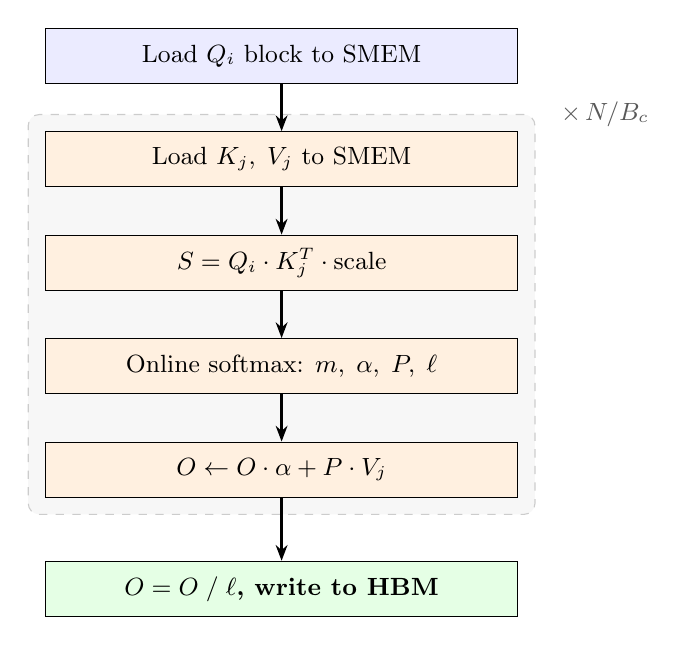
\begin{tikzpicture}[
    node distance=0.6cm,
    block/.style={rectangle, draw, fill=blue!8, minimum width=6cm, minimum height=0.7cm, font=\small},
    op/.style={rectangle, draw, fill=orange!12, minimum width=6cm, minimum height=0.7cm, font=\small},
    res/.style={rectangle, draw, fill=green!10, minimum width=6cm, minimum height=0.7cm, font=\small\bfseries},
    arr/.style={-{Stealth[length=2mm]}, thick},
]

\node[block] (loadq) {Load $Q_i$ block to SMEM};
\node[op, below=of loadq] (loadkv) {Load $K_j,\; V_j$ to SMEM};
\node[op, below=of loadkv] (gemm1) {$S = Q_i \cdot K_j^T \cdot \text{scale}$};
\node[op, below=of gemm1] (softmax) {Online softmax: $m,\; \alpha,\; P,\; \ell$};
\node[op, below=of softmax] (gemm2) {$O \leftarrow O \cdot \alpha + P \cdot V_j$};
\node[res, below=0.8cm of gemm2] (epilogue) {$O = O \;/\; \ell$, write to HBM};

\foreach \a/\b in {loadq/loadkv, loadkv/gemm1, gemm1/softmax, softmax/gemm2, gemm2/epilogue}
    \draw[arr] (\a) -- (\b);

\begin{scope}[on background layer]
\node[fill=gray!6, draw=gray!40, dashed, rounded corners=4pt,
      inner sep=6pt, fit=(loadkv)(gemm1)(softmax)(gemm2)] (loopbox) {};
\end{scope}
\node[font=\small, text=gray!70!black, anchor=west]
    at ($(loopbox.north east)+(0.2,0)$) {$\times\, N / B_c$};

\end{tikzpicture}
\end{center}

\vspace{0.5em}
\tableofcontents
\newpage

%--------------------------------------------------------------
\section{Notation}
%--------------------------------------------------------------

\begin{table}[h]
\centering
\begin{tabular}{@{}clc@{}}
\toprule
\textbf{Symbol} & \textbf{Meaning} & \textbf{Typical Value} \\
\midrule
$N$        & sequence length                    & $1024$--$16384$ \\
$d$        & head dimension                     & 128 \\
$B_r$      & Q block rows (tile height)         & 64 \\
$B_c$      & KV block columns (tile width)      & 32 \\
$S$        & score matrix $QK^T$                & $\R^{N \times N}$ \\
$P$        & attention weight matrix             & $\R^{N \times N}$ \\
$O$        & output matrix                      & $\R^{N \times d}$ \\
$m_i$      & running row max (per row $i$)       & scalar \\
$\ell_i$   & running row sum (per row $i$)       & scalar \\
$\alpha$   & correction factor $e^{m_{\text{old}} - m_{\text{new}}}$ & $\in (0, 1]$ \\
\bottomrule
\end{tabular}
\end{table}

%--------------------------------------------------------------
\section{Standard Attention}
%--------------------------------------------------------------

Given $Q, K, V \in \R^{N \times d}$ where $N$ = sequence length and $d$ = head dimension:

\begin{equation}
S = Q K^T \in \R^{N \times N}
\end{equation}

\begin{equation}
P = \text{softmax}\!\left(\frac{S}{\sqrt{d}}\right) \in \R^{N \times N}
\end{equation}

\begin{equation}
O = P V \in \R^{N \times d}
\end{equation}

Softmax is applied \textbf{row-wise}. For row $i$:

\begin{equation}
m_i = \max_j\!\left(\frac{S_{ij}}{\sqrt{d}}\right), \qquad
\ell_i = \sum_j \exp\!\left(\frac{S_{ij}}{\sqrt{d}} - m_i\right), \qquad
P_{ij} = \frac{\exp\!\left(\frac{S_{ij}}{\sqrt{d}} - m_i\right)}{\ell_i}
\end{equation}

The subtraction by $m_i$ is for numerical stability. It does not change the result:

\begin{equation}
\frac{\exp(x_j - c)}{\sum_k \exp(x_k - c)} = \frac{\exp(x_j)}{\sum_k \exp(x_k)} \quad \text{for any constant } c
\end{equation}

Choosing $c = m_i = \max_j(x_j)$ ensures all exponents are $\leq 0$, preventing overflow.

%--------------------------------------------------------------
\section{Why Naive Attention is Memory-Bound}
%--------------------------------------------------------------

A naive implementation launches three separate kernels, materializing $S$ in HBM between each step:

\begin{table}[h]
\centering
\begin{tabular}{@{}llll@{}}
\toprule
\textbf{Step} & \textbf{Operation} & \textbf{HBM Reads} & \textbf{HBM Writes} \\
\midrule
1 & $S = QK^T$                      & $2Nd$   & $N^2$ \\
2 & $P = \text{softmax}(S/\sqrt{d})$ & $N^2$   & $N^2$ \\
3 & $O = PV$                         & $N^2 + Nd$ & $Nd$ \\
\midrule
\textbf{Total} & & $3N^2 + 3Nd$ & $2N^2 + Nd$ \\
\bottomrule
\end{tabular}
\end{table}

All values in \textbf{elements} (multiply by 2 for FP16 bytes).

\subsection{Concrete Numbers ($N = 4096, \; d = 128$)}

\[
\text{FLOPs} = 4N^2 d = 4 \times 4096^2 \times 128 = 8.59 \;\text{GFLOP}
\]

\[
\text{HBM traffic} \approx 5N^2 \times 2 \;\text{bytes} = 5 \times 4096^2 \times 2 \approx 167 \;\text{MB}
\]

\begin{equation}
\text{Arithmetic Intensity}_{\text{naive}} = \frac{8.59 \;\text{GFLOP}}{0.167 \;\text{GB}} \approx 51 \;\frac{\text{FLOP}}{\text{byte}}
\end{equation}

A100 ridge point (tensor core): $312\;\text{TFLOPS}\;/\;2039\;\text{GB/s} \approx 153$ FLOP/byte. At 51 FLOP/byte, naive attention is \textbf{memory-bound} --- tensor cores are starved waiting for HBM traffic caused by the $N \times N$ intermediate.

%--------------------------------------------------------------
\section{Flash Attention: IO Complexity}
%--------------------------------------------------------------

Flash attention \textbf{never materializes} the $N \times N$ score matrix in HBM. Instead, $S$ is computed tile-by-tile in SMEM/registers, softmax is applied on-the-fly, and the result accumulates directly into $O$.

\begin{table}[h]
\centering
\begin{tabular}{@{}lc@{}}
\toprule
\textbf{Operation} & \textbf{Elements} \\
\midrule
Read $Q$  & $Nd$ \\
Read $K$  & $Nd$ \\
Read $V$  & $Nd$ \\
Write $O$ & $Nd$ \\
\midrule
\textbf{Total} & $4Nd$ \\
\bottomrule
\end{tabular}
\end{table}

\[
\text{HBM traffic} = 4Nd \times 2 = 4 \times 4096 \times 128 \times 2 = 4.19 \;\text{MB}
\]

\begin{equation}
\boxed{
\text{Arithmetic Intensity}_{\text{flash}} = \frac{8.59 \;\text{GFLOP}}{0.00419 \;\text{GB}} \approx 2050 \;\frac{\text{FLOP}}{\text{byte}}
}
\end{equation}

This is $\mathbf{13\times}$ above the ridge point. Flash attention is firmly \textbf{compute-bound}. A $\mathbf{40\times}$ reduction in HBM traffic versus naive.

The $N \times N$ intermediate $S$ now lives entirely in SMEM/registers as small $B_r \times B_c$ tiles. The price: we need a way to compute softmax \textbf{incrementally} without seeing the full row of $S$ at once.

\subsection{Why the $N \times N$ Matrix is the Problem}

Standard attention computes $S = QK^T$ as a full $N \times N$ matrix before softmax can begin:

\begin{center}
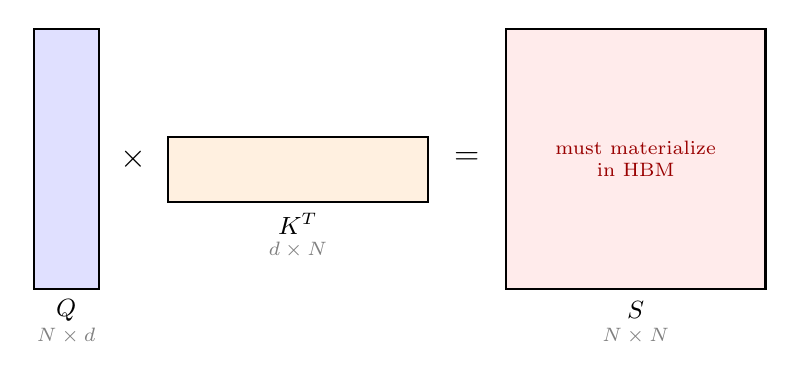
\begin{tikzpicture}[scale=0.55, every node/.style={font=\small}]

    % Q matrix
    \fill[blue!12] (0, 0) rectangle (1.5, 6);
    \draw[thick] (0, 0) rectangle (1.5, 6);
    \node at (0.75, -0.5) {$Q$};
    \node[font=\scriptsize, text=gray] at (0.75, -1.1) {$N \times d$};

    % multiply sign
    \node[font=\large] at (2.3, 3) {$\times$};

    % K^T matrix
    \fill[orange!12] (3.1, 2) rectangle (9.1, 3.5);
    \draw[thick] (3.1, 2) rectangle (9.1, 3.5);
    \node at (6.1, 1.5) {$K^T$};
    \node[font=\scriptsize, text=gray] at (6.1, 0.9) {$d \times N$};

    % equals
    \node[font=\large] at (10, 3) {$=$};

    % S matrix
    \fill[red!8] (10.9, 0) rectangle (16.9, 6);
    \draw[thick] (10.9, 0) rectangle (16.9, 6);
    \node at (13.9, -0.5) {$S$};
    \node[font=\scriptsize, text=gray] at (13.9, -1.1) {$N \times N$};
    \node[font=\scriptsize, text=red!60!black, align=center] at (13.9, 3) {must materialize\\in HBM};

\end{tikzpicture}
\end{center}

Flash attention avoids this by computing $S$ one small tile at a time, applying softmax incrementally, and discarding each tile before computing the next.

\subsection{Tiling Dataflow}

Inside one thread block, processing one $Q$-block across all KV blocks:

\begin{center}
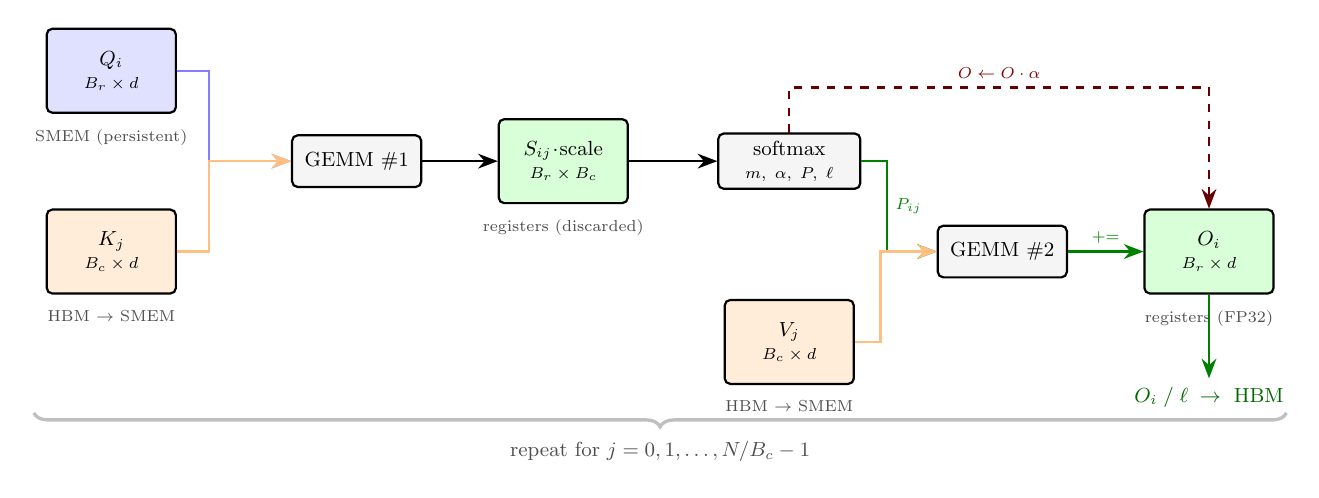
\begin{tikzpicture}[
    scale=0.82, every node/.style={transform shape},
    box/.style={rectangle, draw, thick, minimum height=1.3cm, align=center, font=\small,
                rounded corners=2pt},
    opbox/.style={rectangle, draw, thick, fill=gray!8, minimum width=2cm,
                  minimum height=0.8cm, align=center, font=\small, rounded corners=2pt},
    arr/.style={-{Stealth[length=2.5mm]}, thick},
    mem/.style={font=\scriptsize, text=gray!60!black},
]

    % ── Input blocks ──

    % Q_i (persistent in SMEM)
    \node[box, fill=blue!12, minimum width=2cm] (Q) at (0, 0)
        {$Q_i$\\[-0.1em]{\scriptsize $B_r \times d$}};
    \node[mem, below=0.12cm of Q] {SMEM (persistent)};

    % K_j (streamed from HBM)
    \node[box, fill=orange!15, minimum width=2cm] (K) at (0, -2.8)
        {$K_j$\\[-0.1em]{\scriptsize $B_c \times d$}};
    \node[mem, below=0.12cm of K] {HBM $\to$ SMEM};

    % ── GEMM #1 ──
    \node[opbox] (gemm1) at (3.8, -1.4)
        {GEMM \#1};

    \draw[arr, blue!50] (Q.east) -- ++(0.5,0) |- (gemm1.west);
    \draw[arr, orange!50] (K.east) -- ++(0.5,0) |- (gemm1.west);

    % ── S tile ──
    \node[box, fill=green!15, minimum width=2cm] (S) at (7, -1.4)
        {$S_{ij} \!\cdot\! \text{scale}$\\[-0.1em]{\scriptsize $B_r \times B_c$}};
    \node[mem, below=0.12cm of S] {registers (discarded)};

    \draw[arr] (gemm1.east) -- (S.west);

    % ── Softmax ──
    \node[opbox, minimum width=2.2cm] (sm) at (10.5, -1.4)
        {softmax\\[-0.1em]{\scriptsize $m,\; \alpha,\; P,\; \ell$}};

    \draw[arr] (S.east) -- (sm.west);

    % ── V_j ──
    \node[box, fill=orange!15, minimum width=2cm] (V) at (10.5, -4.2)
        {$V_j$\\[-0.1em]{\scriptsize $B_c \times d$}};
    \node[mem, below=0.12cm of V] {HBM $\to$ SMEM};

    % ── GEMM #2 ──
    \node[opbox] (gemm2) at (13.8, -2.8)
        {GEMM \#2};

    \draw[arr, green!50!black] (sm.east) -- ++(0.4,0) |- node[pos=0.25, right, font=\scriptsize] {$P_{ij}$} (gemm2.west);
    \draw[arr, orange!50] (V.east) -- ++(0.4,0) |- (gemm2.west);

    % ── O accumulator ──
    \node[box, fill=green!15, minimum width=2cm] (O) at (17, -2.8)
        {$O_i$\\[-0.1em]{\scriptsize $B_r \times d$}};
    \node[mem, below=0.12cm of O] {registers (FP32)};

    \draw[arr, green!50!black] (gemm2.east) -- (O.west)
        node[midway, above, font=\scriptsize] {$\mathrel{+}=$};

    % ── Rescale feedback arrow ──
    \draw[arr, red!40!black, dashed] (sm.north) -- ++(0, 0.7) -| (O.north)
        node[pos=0.25, above, font=\scriptsize, text=red!50!black] {$O \leftarrow O \cdot \alpha$};

    % ── Iteration brace ──
    \draw[decorate, decoration={brace, amplitude=5pt, mirror}, very thick, gray!50]
        (-1.2, -5.3) -- (18.2, -5.3);
    \node[font=\small, text=gray!60!black] at (8.5, -5.9) {repeat for $j = 0, 1, \ldots, N/B_c - 1$};

    % ── Final output ──
    \draw[arr, green!50!black] (O.south) -- ++(0, -1.3)
        node[below, font=\small, text=green!40!black] {$O_i \;/\; \ell \;\to\;$ HBM};

\end{tikzpicture}
\end{center}

$Q_i$ stays in SMEM for the entire loop. Each iteration streams one $K_j, V_j$ pair from HBM, computes the $B_r \times B_c$ score tile in registers (never written to HBM), applies online softmax with the $\alpha$ correction to $O$, and accumulates $P_{ij} V_j$ via GEMM \#2. After all KV blocks, $O_i$ is divided by $\ell$ and written to HBM once.

%--------------------------------------------------------------
\section{Online Softmax}
%--------------------------------------------------------------

Standard softmax is a \textbf{two-pass} algorithm:
\[
\text{Pass 1: } m = \max(x_1, \ldots, x_N) \qquad \text{Pass 2: } \ell = \sum_{j} \exp(x_j - m), \quad y_j = \frac{\exp(x_j - m)}{\ell}
\]

This requires the \textbf{entire row}. In flash attention, we only have $B_c$ elements at a time. We need to compute $m$ and $\ell$ incrementally.

\subsection{Derivation}

Suppose we have processed block $A$ (first $B_c$ elements) and have:
\[
m_A = \max_{j \in A}(x_j), \qquad \ell_A = \sum_{j \in A} \exp(x_j - m_A)
\]

Now block $B$ (next $B_c$ elements) arrives. The new global max is:
\[
m_{\text{new}} = \max(m_A, \; \max_{j \in B}(x_j))
\]

The old terms were computed with base $m_A$. We need to \textbf{re-base} them to $m_{\text{new}}$:
\[
\exp(x_j - m_A) \cdot \underbrace{\exp(m_A - m_{\text{new}})}_{\alpha} = \exp(x_j - m_{\text{new}})
\]

Define the \textbf{correction factor}:
\begin{equation}
\boxed{\alpha = \exp(m_{\text{old}} - m_{\text{new}})}
\end{equation}

Since $m_{\text{new}} \geq m_{\text{old}}$, we have $\alpha \leq 1$ --- always scaling \textbf{down}, numerically stable.

The updated running sum:
\begin{equation}
\boxed{\ell_{\text{new}} = \ell_{\text{old}} \cdot \alpha + \sum_{j \in B} \exp(x_j - m_{\text{new}})}
\end{equation}

\textbf{Proof:}
\[
\ell_{\text{new}} = \sum_{j \in A \cup B} \exp(x_j - m_{\text{new}})
= \underbrace{\sum_{j \in A} \exp(x_j - m_A)}_{\ell_A} \cdot \alpha + \sum_{j \in B} \exp(x_j - m_{\text{new}})
= \ell_A \cdot \alpha + \sum_{j \in B} \exp(x_j - m_{\text{new}}) \;\; \checkmark
\]

\subsection{Output Accumulator Rescaling}

We maintain a running \textbf{unnormalized} output accumulator:
\[
O_{\text{unnorm}} = \sum_{j \;\text{seen}} \exp(x_j - m_{\text{current}}) \cdot v_j
\]

When the max changes, every previous term needs re-basing by the same factor $\alpha$:
\begin{equation}
\boxed{O_{\text{new}} = O_{\text{old}} \cdot \alpha + \underbrace{\sum_{j \in B} \exp(x_j - m_{\text{new}}) \cdot v_j}_{P_{\text{block}} \;\times\; V_{\text{block}}}}
\end{equation}

The second term is a \textbf{matrix multiply}: the exponentiated scores $P_{\text{block}}$ times the value matrix $V_{\text{block}}$.

After all blocks: $O_{\text{final}} = O_{\text{unnorm}} \;/\; \ell$.

\subsection{Worked Example}

Let $\vect{x} = [1,\; 0,\; 2,\; 0]$ split into blocks $A = [1,\; 0]$ and $B = [2,\; 0]$.

\medskip
\noindent\textbf{Standard (needs entire row):}

$m = 2, \quad \ell = e^{-1} + e^{-2} + e^{0} + e^{-2} = 0.368 + 0.135 + 1.0 + 0.135 = 1.638$

\medskip
\noindent\textbf{Online (streaming):}

\begin{tabular}{@{}p{1.5cm}p{12cm}@{}}
\textit{Init:} & $m = -\infty, \quad \ell = 0$ \\[0.5em]
\textit{Block A:} & $m_{\text{new}} = \max(-\infty, 1, 0) = 1$ \\
 & $\alpha = e^{-\infty - 1} = 0$ \quad (first block, no history to correct) \\
 & $\ell = 0 \cdot 0 + e^{1-1} + e^{0-1} = 1.0 + 0.368 = 1.368$ \\
 & $m = 1$ \\[0.5em]
\textit{Block B:} & $m_{\text{new}} = \max(1, 2, 0) = 2$ \\
 & $\alpha = e^{1 - 2} = 0.368$ \quad {\color{red!70!black}(max changed --- rescale)} \\
 & $\ell = 1.368 \cdot 0.368 + e^{2-2} + e^{0-2} = 0.503 + 1.0 + 0.135 = \mathbf{1.638}$ \;\checkmark \\
 & $O = O_{\text{old}} \cdot 0.368 + P_B \cdot V_B$ \\
 & $m = 2$ \\
\end{tabular}

\medskip
Both produce $\ell = 1.638$. The online version corrected its previous work by $\alpha = 0.368$ when the max changed.

\subsection{State Evolution Across KV Blocks}

\begin{center}
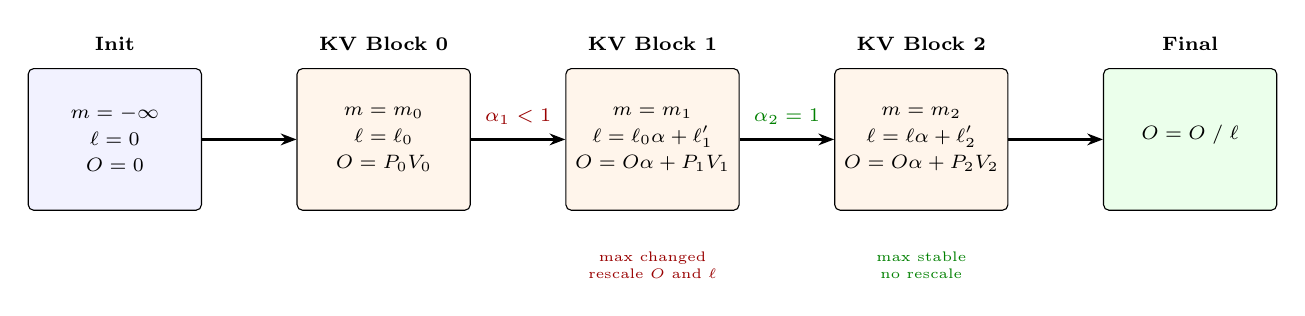
\begin{tikzpicture}[
    state/.style={rectangle, draw, fill=#1, minimum width=2.2cm, minimum height=1.8cm,
                  font=\scriptsize, align=center, rounded corners=2pt},
    state/.default={gray!5},
    arr/.style={-{Stealth[length=2mm]}, thick},
    alabel/.style={font=\scriptsize, text=red!60!black, fill=white, inner sep=1pt},
    alabelg/.style={font=\scriptsize, text=green!50!black, fill=white, inner sep=1pt},
]

\node[state=blue!5] (init) {
    $m = -\infty$\\[0.2em]
    $\ell = 0$\\[0.2em]
    $O = 0$
};
\node[font=\scriptsize\bfseries, above=0.1cm of init] {Init};

\node[state=orange!8, right=1.2cm of init] (kv0) {
    $m = m_0$\\[0.2em]
    $\ell = \ell_0$\\[0.2em]
    $O = P_0 V_0$
};
\node[font=\scriptsize\bfseries, above=0.1cm of kv0] {KV Block 0};

\node[state=orange!8, right=1.2cm of kv0] (kv1) {
    $m = m_1$\\[0.2em]
    $\ell = \ell_0 \alpha + \ell_1'$\\[0.2em]
    $O = O\alpha + P_1 V_1$
};
\node[font=\scriptsize\bfseries, above=0.1cm of kv1] {KV Block 1};

\node[state=orange!8, right=1.2cm of kv1] (kv2) {
    $m = m_2$\\[0.2em]
    $\ell = \ell \alpha + \ell_2'$\\[0.2em]
    $O = O\alpha + P_2 V_2$
};
\node[font=\scriptsize\bfseries, above=0.1cm of kv2] {KV Block 2};

\node[state=green!8, right=1.2cm of kv2] (final) {
    \\[0.2em]
    $O = O \;/\; \ell$\\[0.2em]
};
\node[font=\scriptsize\bfseries, above=0.1cm of final] {Final};

\draw[arr] (init) -- (kv0);
\draw[arr] (kv0) -- (kv1) node[midway, alabel, above=4pt] {$\alpha_1 < 1$};
\draw[arr] (kv1) -- (kv2) node[midway, alabelg, above=4pt] {$\alpha_2 = 1$};
\draw[arr] (kv2) -- (final);

\node[font=\tiny, text=red!60!black, below=0.4cm of kv1, align=center] {max changed\\rescale $O$ and $\ell$};
\node[font=\tiny, text=green!50!black, below=0.4cm of kv2, align=center] {max stable\\no rescale};

\end{tikzpicture}
\end{center}

\begin{itemize}[leftmargin=1.5em, itemsep=0.3em]
\item $\alpha$ is a per-row \textbf{scalar} applied to a \textbf{matrix} $O$ --- cheap rescale of expensive accumulator.
\item Once the running max stabilizes (common after a few blocks), $\alpha = 1$ and no rescale is needed.
\item The denominator $\ell$ is only used at the very end --- we carry unnormalized $O$ throughout.
\end{itemize}

%--------------------------------------------------------------
\section{The Complete Update Rule}
%--------------------------------------------------------------

At each KV block $j$, for each query row $i$:

\begin{equation}
\boxed{
\begin{aligned}
S_j &= Q_i \; K_j^T & & \text{(GEMM \#1)} \\
m_{\text{new}} &= \max(m, \;\text{rowmax}(S_j / \sqrt{d})) & & \text{(per-row max)} \\
\alpha &= \exp(m - m_{\text{new}}) & & \text{(correction, } \leq 1 \text{)} \\
P_j &= \exp(S_j / \sqrt{d} - m_{\text{new}}) & & \text{(element-wise)} \\
\ell &\leftarrow \ell \cdot \alpha + \text{rowsum}(P_j) & & \text{(update denominator)} \\
O &\leftarrow O \cdot \alpha + P_j \; V_j & & \text{(GEMM \#2 + rescale)} \\
m &\leftarrow m_{\text{new}} & &
\end{aligned}
}
\end{equation}

Initialization: $m = -\infty, \;\; \ell = 0, \;\; O = 0$. \quad Finalization: $O = O \;/\; \ell$.

\subsection{Algorithmic Verification (Python)}

\begin{lstlisting}[style=python]
for kv_start in range(0, N, Bc):
    K_block = K[kv_start : kv_start + Bc]   # [Bc, d]
    V_block = V[kv_start : kv_start + Bc]   # [Bc, d]

    S = Q_block @ K_block.T * scale          # GEMM #1: [Br, Bc]

    m_new = np.maximum(m, S.max(axis=1))     # per-row max
    alpha = np.exp(m - m_new)                # correction factor

    P = np.exp(S - m_new[:, None])           # exponentiate

    l = l * alpha + P.sum(axis=1)            # update denominator
    O = O * alpha[:, None] + P @ V_block     # GEMM #2 + rescale

    m = m_new

O_final = O / l[:, None]                     # normalize
\end{lstlisting}

%--------------------------------------------------------------
\section{Causal Masking}
%--------------------------------------------------------------

In autoregressive models, token $i$ can only attend to tokens $j \leq i$. This is enforced by a \textbf{lower-triangular mask}:
\[
\tilde{S}_{ij} =
\begin{cases}
S_{ij} & \text{if } j \leq i \\
-\infty & \text{if } j > i
\end{cases}
\]

Since $\exp(-\infty) = 0$, masked positions contribute nothing to $\ell$ or $O$. The online softmax algorithm requires \textbf{zero changes}.

\subsection{Block-Level Classification}

The Q block covers rows $[q,\; q + B_r)$ and the KV block covers columns $[k,\; k + B_c)$. Three cases:
\begin{align}
q + B_r \leq k &\implies \text{entire tile is masked} \rightarrow \textbf{skip} \\
q \geq k + B_c &\implies \text{entire tile is visible} \rightarrow \textbf{full} \\
\text{otherwise} &\implies \text{diagonal tile} \rightarrow \textbf{element-wise mask}
\end{align}

\begin{center}
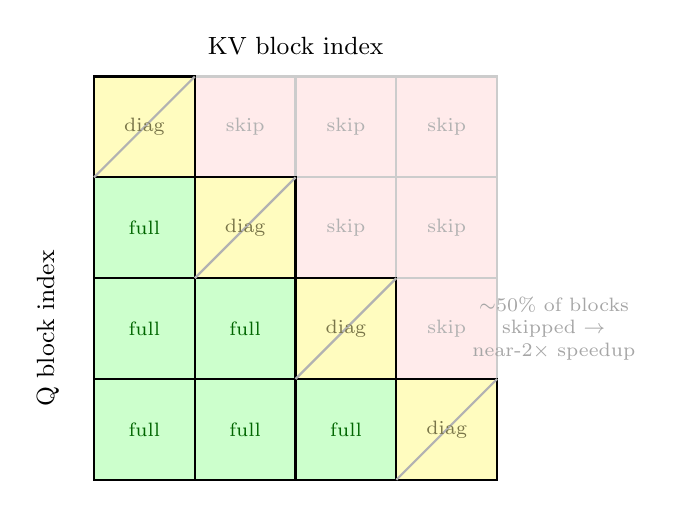
\begin{tikzpicture}[scale=0.8]
    \def\bs{1.6}

    % Lower triangle = full (green)
    \foreach \r/\c in {1/0, 2/0, 2/1, 3/0, 3/1, 3/2} {
        \fill[green!20] (\c*\bs, -\r*\bs) rectangle +(\bs, \bs);
        \draw[thick] (\c*\bs, -\r*\bs) rectangle +(\bs, \bs);
        \node[font=\scriptsize, green!40!black] at (\c*\bs+\bs/2, -\r*\bs+\bs/2) {full};
    }

    % Upper triangle = skip (red/gray)
    \foreach \r/\c in {0/1, 0/2, 0/3, 1/2, 1/3, 2/3} {
        \fill[red!8] (\c*\bs, -\r*\bs) rectangle +(\bs, \bs);
        \draw[thick, gray!40] (\c*\bs, -\r*\bs) rectangle +(\bs, \bs);
        \node[font=\scriptsize, gray!60] at (\c*\bs+\bs/2, -\r*\bs+\bs/2) {skip};
    }

    % Diagonal (yellow)
    \foreach \r in {0, 1, 2, 3} {
        \fill[yellow!25] (\r*\bs, -\r*\bs) rectangle +(\bs, \bs);
        \draw[thick] (\r*\bs, -\r*\bs) rectangle +(\bs, \bs);
        \draw[thick, gray!60] (\r*\bs, -\r*\bs) -- (\r*\bs+\bs, -\r*\bs+\bs);
        \node[font=\scriptsize, yellow!40!black] at (\r*\bs+\bs/2, -\r*\bs+\bs/2) {diag};
    }

    % Axis labels
    \node[font=\small, above] at (2*\bs, \bs+0.2) {KV block index};
    \node[font=\small, rotate=90, anchor=south] at (-0.4, -1.5*\bs) {Q block index};

    % Annotation
    \node[font=\scriptsize, text=gray!70, align=center] at (3*\bs+2.5, -1.5*\bs)
        {$\sim$50\% of blocks\\skipped $\rightarrow$\\near-2$\times$ speedup};
\end{tikzpicture}
\end{center}

Skipping upper-triangle blocks avoids $\sim N^2/2$ elements of unnecessary compute. The element-wise mask on a diagonal block sets $S[\text{local\_q}][\text{local\_k}] = -\infty$ wherever global\_q $<$ global\_k.

%--------------------------------------------------------------
\section{CUDA Core Implementation}
%--------------------------------------------------------------

This section maps the algorithm to a self-contained CUDA kernel using pure scalar FP32 arithmetic. No tensor cores, no MMA, no \texttt{ldmatrix}, no \texttt{cp.async} --- just \texttt{FMUL} + \texttt{FADD} on CUDA cores. The kernel is a readable reference, not a performance target.

Source: \texttt{src/cuda\_core\_reference.cu}.

\subsection{Thread and Block Mapping}

One thread per output row. $\texttt{NUM\_THREADS} = B_r$. Each thread independently computes its row's QK dots, softmax, and PV accumulation. Threads cooperate only on SMEM loads.

\begin{lstlisting}
template<int BR, int BC, int D>
__global__ void flash_cuda_core(
    const __half* __restrict__ Q,
    const __half* __restrict__ K,
    const __half* __restrict__ V,
    __half* __restrict__ O,
    int N)
{
    const float SCALE = 1.0f / sqrtf((float)D);

    int tid   = threadIdx.x;       // row index within Q-block
    int q_blk = blockIdx.x;       // which Q-block
    int head  = blockIdx.y;
    int batch = blockIdx.z;

    int base = (batch * gridDim.y + head) * N * D;
\end{lstlisting}

Grid: \texttt{dim3(N/BR, n\_heads, batch)}. Each block processes one $B_r \times d$ output tile.

\subsection{SMEM Layout}

All shared memory is FP32. FP16 $\to$ FP32 conversion happens at the GMEM/SMEM boundary.

\begin{equation}
\text{SMEM} = \underbrace{B_r \times d}_{Q} + \underbrace{B_c \times d}_{K} + \underbrace{B_c \times d}_{V} = (B_r + 2 B_c) \times d \times 4 \;\text{bytes}
\end{equation}

For $B_r = 64, B_c = 32, d = 128$: $(64 + 64) \times 128 \times 4 = 64$\,KB.

\begin{lstlisting}
    extern __shared__ float smem[];
    float* sQ = smem;                     // [BR x D]
    float* sK = smem + BR * D;            // [BC x D]
    float* sV = smem + (BR + BC) * D;     // [BC x D]

    // Load Q tile once: GMEM (FP16) -> SMEM (FP32)
    for (int i = tid; i < BR * D; i += BR)
        sQ[i] = __half2float(Q_tile[i]);
    __syncthreads();
\end{lstlisting}

$Q$ is loaded once and reused for every KV block. $K$ and $V$ are overwritten each iteration.

\subsection{Per-Thread Accumulators}

Direct mapping to the math: \texttt{O\_acc[D]} $\leftrightarrow O$, \quad \texttt{m} $\leftrightarrow m$, \quad \texttt{l} $\leftrightarrow \ell$.

\begin{lstlisting}
    float O_acc[D];
    for (int d = 0; d < D; d++)
        O_acc[d] = 0.0f;             // O = 0
    float m = -INFINITY;              // m = -inf
    float l = 0.0f;                   // l = 0
\end{lstlisting}

\subsection{Main Loop}

Each phase maps directly to the update rule from Section~6.

\begin{lstlisting}
    int n_kv = N / BC;

    for (int j = 0; j < n_kv; j++) {

        // Cooperative load K[BC x D] and V[BC x D]
        const __half* Kj = K_head + j * BC * D;
        const __half* Vj = V_head + j * BC * D;
        for (int i = tid; i < BC * D; i += BR) {
            sK[i] = __half2float(Kj[i]);
            sV[i] = __half2float(Vj[i]);
        }
        __syncthreads();
\end{lstlisting}

\medskip
\noindent\textbf{Phase 1} --- $S_j = Q_i K_j^T / \sqrt{d}$, \; $m_{\text{new}} = \max(m, \text{rowmax}(S_j))$

\begin{lstlisting}
        float S[BC];
        float new_max = m;
        for (int c = 0; c < BC; c++) {
            float dot = 0.0f;
            for (int d = 0; d < D; d++)
                dot += sQ[tid * D + d] * sK[c * D + d];
            S[c] = dot * SCALE;
            new_max = fmaxf(new_max, S[c]);
        }
\end{lstlisting}

Each thread computes its row's dot product with all $B_c$ key vectors. The inner loop over \texttt{D} is the contraction dimension of GEMM \#1. Row max is found in the same pass.

\medskip
\noindent\textbf{Phase 2} --- $\alpha = \exp(m_{\text{old}} - m_{\text{new}})$, \; $O \leftarrow O \cdot \alpha$, \; $\ell \leftarrow \ell \cdot \alpha$

\begin{lstlisting}
        float alpha = __expf(m - new_max);
        for (int d = 0; d < D; d++)
            O_acc[d] *= alpha;
        l *= alpha;
        m = new_max;
\end{lstlisting}

When $m$ does not change, $\alpha = 1$ and this is a no-op.

\medskip
\noindent\textbf{Phase 3} --- $P_j = \exp(S_j - m)$, \; $\ell \mathrel{+}= \text{rowsum}(P_j)$, \; $O \mathrel{+}= P_j V_j$

\begin{lstlisting}
        for (int c = 0; c < BC; c++) {
            float p = __expf(S[c] - m);
            l += p;
            for (int d = 0; d < D; d++)
                O_acc[d] += p * sV[c * D + d];
        }

        __syncthreads();
    }
\end{lstlisting}

The inner loop over \texttt{D} is GEMM \#2, unrolled: for each column $c$ of $P$, we scale $V_j[c, :]$ by $P[c]$ and accumulate into $O$. The \texttt{\_\_syncthreads()} at the bottom protects SMEM before the next KV block overwrites it.

\subsection{Epilogue}

\begin{lstlisting}
    float inv_l = 1.0f / l;
    for (int d = 0; d < D; d++)
        O_tile[tid * D + d] = __float2half(O_acc[d] * inv_l);
}
\end{lstlisting}

Normalize $O$ by $\ell$, convert FP32 $\to$ FP16, write to GMEM. Each thread writes its own row.

\subsection{Resource Budget}

\begin{table}[h]
\centering
\begin{tabular}{@{}lcr@{}}
\toprule
\textbf{Item} & \textbf{Type} & \textbf{Cost} \\
\midrule
\texttt{O\_acc[D]} & $d$ floats in registers         & 128 regs \\
\texttt{S[BC]}     & $B_c$ floats in registers        & 32 regs \\
\texttt{m, l, alpha, p, dot, ...} & scalars          & $\sim$10 regs \\
\midrule
\textbf{Total per thread} & & $\sim$170 / 255 max \\
\midrule
\texttt{sQ[BR $\times$ D]}     & SMEM (FP32)    & 32\,KB \\
\texttt{sK[BC $\times$ D]}     & SMEM (FP32)    & 16\,KB \\
\texttt{sV[BC $\times$ D]}     & SMEM (FP32)    & 16\,KB \\
\midrule
\textbf{Total SMEM} & & \textbf{64\,KB} \\
\bottomrule
\end{tabular}
\caption*{$B_r = 64, \; B_c = 32, \; d = 128$.}
\end{table}

%--------------------------------------------------------------
\section{Summary}
%--------------------------------------------------------------

\begin{table}[h]
\centering
\begin{tabular}{@{}ll@{}}
\toprule
\textbf{Concept} & \textbf{Key Equation / Code} \\
\midrule
Standard attention     & $O = \text{softmax}(QK^T / \sqrt{d}) \cdot V$ \\
Naive AI               & $\sim 51$ FLOP/byte (memory-bound) \\
Flash AI               & $\sim 2050$ FLOP/byte (compute-bound) \\
Correction factor      & $\alpha = \exp(m_{\text{old}} - m_{\text{new}})$ \;\;$\to$\;\; \texttt{\_\_expf(m - new\_max)} \\
Running sum            & $\ell \leftarrow \ell \cdot \alpha + \text{rowsum}(P)$ \;\;$\to$\;\; \texttt{l = l*alpha + ...} \\
Output rescale         & $O \leftarrow O \cdot \alpha + P V$ \;\;$\to$\;\; \texttt{O\_acc[d] *= alpha; O\_acc[d] += p*sV[...]} \\
Causal block skip      & skip if $q_{\text{off}} + B_r \leq k_{\text{off}}$ \\
SMEM footprint         & $(B_r + 2B_c) \times d \times 4$ bytes \\
Register budget        & $\sim d + B_c + 10$ floats per thread \\
\bottomrule
\end{tabular}
\end{table}

\end{document}
